
\subsection{Power Budget}
\indent After analyzing the power consumption of the individual components of the sensor package, the following power budget was formed (Table \ref*{tab:PowerBudget}). Note that there was $+10\%$ allocation added to the total power calculated. This was to account for any errors in calculation or any miscellaneous items that were looked over. 

\begin{table}
\centering
\begin{tabular}{|l|l|}\hline
Component & Power Consumption (mW)\\\hline
Beagle Bone Black & 2300\\\hline
Analog to Digital Converter & 0.66\\\hline
GPS & 132\\\hline
Wireless Transmitter(Anticipated) & 800\\\hline
Strain Gauge & 95\\\hline
Accelerometer & 1320\\\hline
Total Power & 4650\\
\hline

\end{tabular}
\caption{\textit{Time without power production}}
\label{tab:PowerBudget}
\end{table}

\indent After adjusting the power budget to a more conservative value, the package is projected to be a 5 Watt system. By specifying a constant power consumption, an ideal battery capacity can be determined. The power values calculated for each component were under the assumption that the system would run continuously. In the future implementation of a wireless transmitter, a constant current draw of 215 mA was assumed. This value corresponds to a maximum power consumption and does not account for a possible boost in signal. 


\subsection{Package Power}

\subsubsection{Solar Potential}

\indent The design of a sensor package with multiple instruments requires careful planning in order for each piece to work properly and accurately. Creating a package that continuously takes measurements and wirelessly transmits this data raises the question of how to power the system. The package is designed for long term structural health monitoring, making energy storage imperative.  Energy can be scavenged in a number of ways; the popular methods depend on the more abundant natural resources, solar and wind energy. The energy scavenging devices essential to this project are a solar panel, wind turbine, and rechargeable battery system.\\

\indent The National Oceanic and Atmospheric Administration  is a scientific agency that is a part of the U.S. department of commerce. Through the Earth System Research Laboratory, NOAA offers datasets for various climate properties such as humidity, temperature, cloud coverage, etc. The statistical analysis of hind-cast data is crucial for the design of an energy storage system. NOAA offers data for the downward short wave radiation flux for the past 65 years. These files can be imported into MATLAB and refined for the values relevant to a desired location. The data is recorded for all locations around the world based on the respective longitude and latitude, Newport, Rhode Island is located at latitude (41.5), longitude (-71.3). \\

\indent One year of data will show the trend of available sunlight throughout the change of seasons. It is necessary to take into account periods of time with limited sunlight such as an overcast lasting multiple days. In order to account for events of negligible sunlight over the years, solar data from 1994 through 2013 was uploaded. By averaging each daily average value over the last 20 years, a plot of expected solar radiation flux was generated for a given year. Downward short wave radiation flux is a measure of power in units of Watts per square meter, this data is illustrated in the figure below.

\begin{figure}[H]
\centering
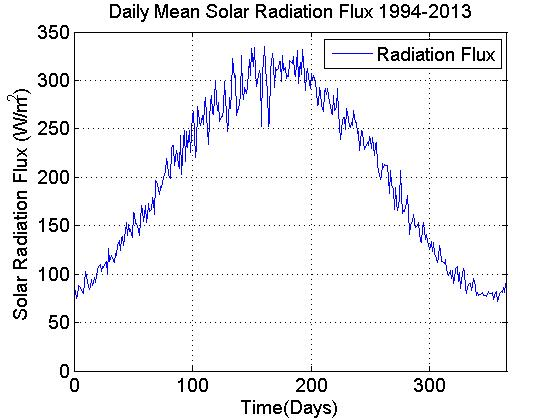
\includegraphics[width=0.7\textwidth]{NewportRadiation.jpg}
\caption{Newport Radiation}
\label{fig:NewportRadtiation}
\end{figure}

\indent To determine the amount of power that can be generated from a given solar panel, the power rating must be used. This project used two, five watt photo-voltaic solar panels purchased from SunForce. Solar panels have a power rating that is directly proportional to their surface area. In order to convert radiation flux, measured in watts per square meter, to the power outputted by a solar panel, the efficiency factor of the panel must be calculated.

\indent Solar cell efficiencies are measured conventionally under standard test conditions that correspond to a clear day with incident solar radiation. These standard conditions specify a test environment with temperature of 25 degrees Celsius and direct radiation flux of 1000 watts per square meter. The ratio of the specific power rating to the radiation flux in standard conditions yields the efficiency factor, which has units of square meters. Multiplying a value of actual radiation flux that the solar panel may experience by the efficiency factor will determine the expected power output of the panel in units of Watts.
\begin{equation}
Efficiency Factor=(\frac{Power Rating}{(\frac{1000W}{m^2})})\
\end{equation}
\indent This calculation can be done for the average solar radiation flux over the past 20 years which is approximately 199.7 watts per square meter. Therefore, the average expected output power from a 5 watt solar panel is one watt. By implementing both solar panels in parallel, the output power doubles, hence the expected output power is 2 watts. Figure 2 shown below illustrates the output power throughout a period of 365 days as well as plotting each daily average power minus one standard deviation. Conceptually, this statistical analysis will yield a more realistic and conservative range of output power. 
\begin{figure}[H]
\centering
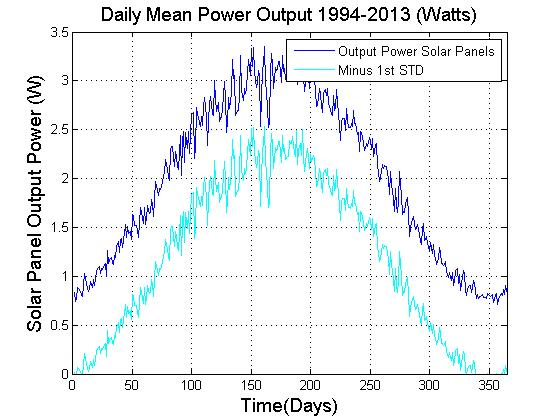
\includegraphics[width=0.7\textwidth]{SolarPanel.jpg}
\caption{\textit{SolarPanel}}
\label{fig:SolarPanel}
\end{figure}

\indent Orientation of a solar panel depends on two things, the inclination from the horizontal, and the direction at which the solar panel faces. As a rule of thumb, a solar panel mounted in the northern hemisphere should be directed true south, and in the southern hemisphere directed north. For optimal performance, the tilt of the solar panel should be adjusted seasonally to obtain the most energy over a whole year. For this project, it was assumed that the solar panels stay at a fixed tilt. To determine the optimal tilt above the horizontal, most articles suggest an inclination equal to the latitude, for Newport that would be 41 degrees. As previously stated, the tilt should be adjusted twice a year during the change of seasons. For the winter months, the angle should equal the latitude plus fifteen degrees, while in the summer time being angled at the latitude minus fifteen degrees. Since this is a hybrid energy scavenging system, the wind turbine will be working in tandem with the solar panels and it is expected that a majority of the energy will be gathered by the wind turbine. For that fact, the solar panels should be oriented for optimal performance during the summer season, when the wind turbine experiences the lowest wind speeds.  




\section{Battery Selection}
\indent The factors that were important in selection of a battery for energy storage were the size and specific battery chemistry. Each battery chemistry such as lead acid, nickel metal hydride or lithium ion, have certain advantages over one another depending on the application. Most energy scavenging systems use lead acid as they are more straight forward and simple to recharge. Lead acid batteries  however are larger bulkier than others such as Lithium Polymer. For that reason, the battery chemistry used in this project for energy storage were Lithium Polymer.  Other properties to take into account when selecting a battery are the energy density as well as the number of recharge cycles one can get out of the battery. The figure below is an illustration of mass and volume energy densities specific to the various battery chemistries. It is clear that lead acid and lithium polymer reside on opposite ends of the plot. 
\indent Lithium Polymer batteries are exceptionally useful in applications that have space limitations such as remote operated vehicles. For this project, all of the hardware must fit inside of a case for weather proofing, making "LiPo" a reasonable selection for rechargeable battery. Another advantage to using Lithium Polymer is that they can be made into any shape or size. 
\indent Using the power budget listed above, which highlights the power consumption relative to each piece of the package, A battery was selected. To be conservative, the power budget was doubled, making the package a 6 Watt system. It was determined that in a worst case scenario, the rechargeable battery must be capable of powering the package for a minimum of 3 days. After researching various capacities of batteries, two 12 AmpHour Lithium Ion batteries were purchased. The purchase of lithium ion over lithium polymer was due to misunderstanding, however testing was still carried out in order to generate discharge curves. In the future progress of this project, the design of a charge controller capable of accepting both solar and wind as well as being able to manage the charge of lithium polymer batteries must be implemented. In order to use battery chemistries such as lithium polymer/ion coupled with such a high power wind turbine, a charge controller is paramount. 

\begin{figure}
\centering
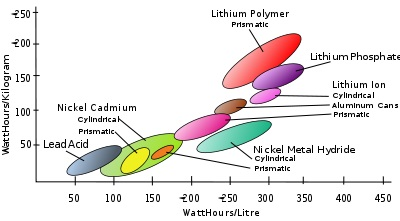
\includegraphics[width=\linewidth]{Battery_Chemistry}
\caption{\textit{Mass and Volume Energy Densities for Various Battery Chemistries}}
\label{fig:Battery_Chemistry}
\end{figure}
